\section{Base Architecture}

\subsection{Transformer}
The T5 model is largely based on the transformer architecture which was first introduced in “Attention is all you need” paper by Vaswani et al. The transformer architecture proposes to use attention mechanism as a replacement for then prevalent recurrent and convolution neural network to identify dependency between input and output tokens. 
\begin{figure}[H]
\centering
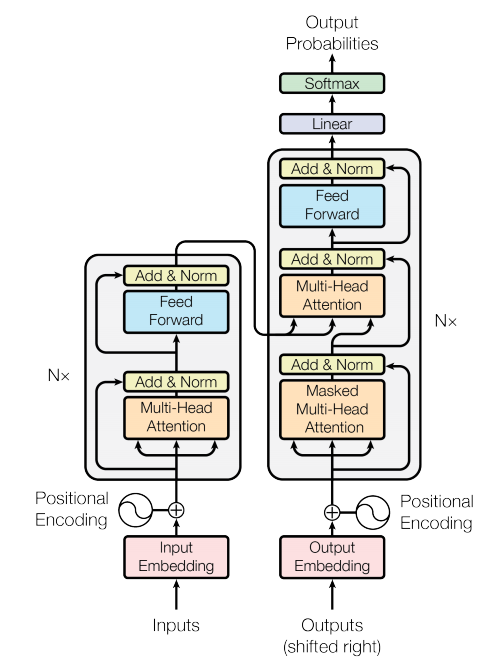
\includegraphics[width=0.7\textwidth]{images/transformer.png}
\caption{Transformer architecture}
\label{fig:transformer}
\end{figure}

The architecture consists of N stacked encoder followed by N stacked decoder layers. Each encoder layer consists of Multi head attention layer followed by feed forward layer, where the output from each of these layer passes through a layer normalisation. The decoder layer consists of the same components as encoder in addition to the masked multi head attention on the output tokens. Both the input and output tokens are vectorised by word2vec embedding and position of the tokens are encoded by a set of sine and cosine functions. The output from the decoder is then passed through a linear layer with SoftMax activation function to get the final results. 

\subsubsection{Attention}
In a traditional sequence model setting such as RNN or LSTM, there is a single context vector that captures the entire information of the input sentence. This context vector (or) hidden layer is used to generate output in the decoder layer. In case of sequence to sequence model, the context vector is passed through the decoder layer where it further encodes the decoder tokens at previous timesteps. This method works well for small sentences. \\
As the length of the sentence increases, the context vector is unable to encode all the information of the sentence in an efficient manner. \\
\begin{figure}[H]
\centering
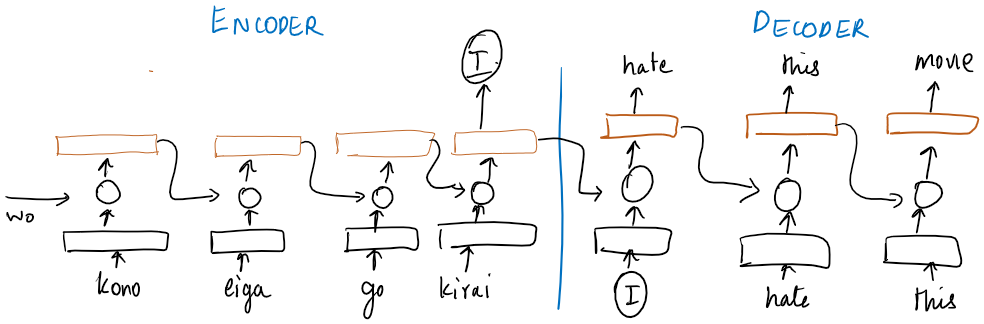
\includegraphics[width=0.9\textwidth]{images/rnn.png}
\caption{Encoder-decoder model}
\label{fig:rnn}
\end{figure}

Attention mechanism (Figure 3) weighs each term of sequence by focusing on relevant part of the sequence. The context vector of each token at decoder layer is calculated based on the contribution of each input token. Thus, the context vector encodes only relevant information at each time step. This enables it to process long sentences effectively and further preventing the vanishing gradient problem

\begin{figure}[H]
\centering
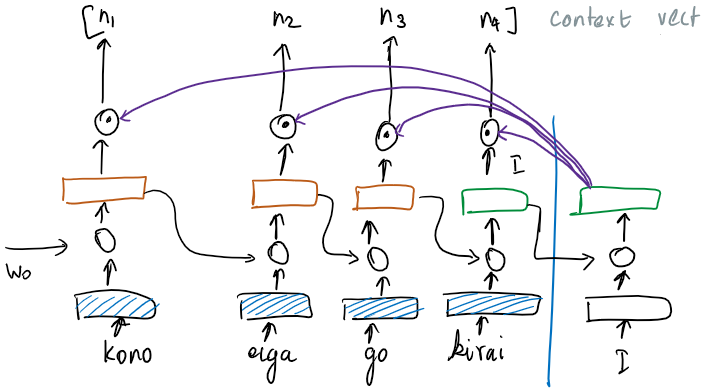
\includegraphics[width=0.7\textwidth]{images/attn.png}
\caption{Attention mechanism}
\label{fig:attn}
\end{figure} 
The Attention is computed from the formula \\
\(Attention(Q,K,V) = softmax((Q.K^{T})/ \sqrt{ d_{k} }).V\)
\\ Where K, V are the key value pair representing the encoder hidden state and Query Q represents the decoder hidden state

\subsubsection{Multi head attention}
Attention mechanism in both encoding and decoding layer is performed as Multi-head Attention. It helps to focus not just on different words in a sentence but also on different segments of the words. Each sentence is divided into h different blocks and attention is performed on each of these blocks. This step can be easily parallelized and the final representation of the sequence is the concatenation of result from each of these blocks.  \\
The output tokens are attended by Masked Multi head attention. It is essentially attention with Mask vector to ensure terms attend only to itself and previous time step terms. 

\begin{figure}[H]
\centering
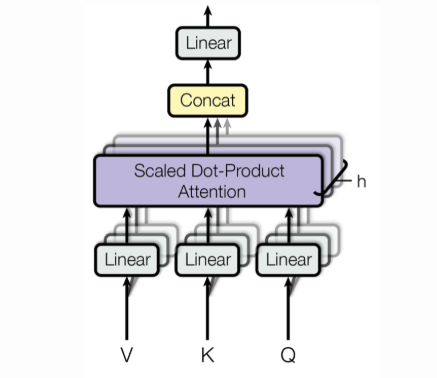
\includegraphics[width=0.4\textwidth]{images/mutlihead.png}
\caption{Multi head attention}
\label{fig:multihead}
\end{figure} 

\subsubsection{Self attention}
The Multi head attention at encoding layer and Masked multi head attention at decoder layer performs Self-attention. Self-attention is similar to attention mechanism where both Query and Key, Value pair are same. Thus, it can be seen as a representation of the sequence by relating different positions of a single sequence.
\begin{figure}[H]
\centering
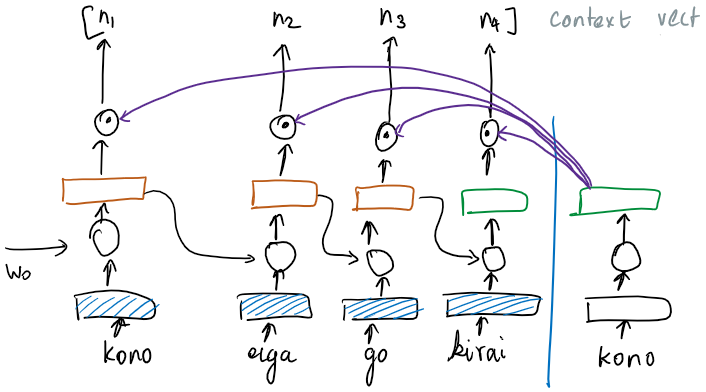
\includegraphics[width=0.7\textwidth]{images/selfattn.png}
\caption{Self Attention}
\label{fig:selfattn}
\end{figure} 

\subsection{Text-to-Text Transfer Transformer}
The Text to text transfer transformer, hence the name T5, model is a Transformer that takes text as an input and returns text as output. The input text consists of prefix that represents task objective such as sentence similarity or sentiment classification followed by the original text input. The output of the NLP tasks which maybe a classification output, number or part of the input text are also modelled in text format. As an example, In case of machine translation task, \\
The input text is “translate Japanese to English: Kono eiga ga kirai”\\
The output text is “I hate this movie”

\subsubsection{Architecture}
The T5 model consists of same transformer model that was discussed earlier except for following changes,
\begin{enumerate}
\item At the layer normalisation, the bias is removed and the it is placed outside the residual skip connection
\item The position of the tokens in the sequence are encoded based on the relative position from one another. 
\item Word piece embedding that considers combination of word vectors and character encoding from a fixed vocabulary instead of word2vec. 
\end{enumerate}
It consists of 12 layers of encoder and decoder layers followed by a feed forward layer with output layer of 3072 dimensionality and dropout layer with dropout probability of 0.1, 12 attention heads. Together the baseline model has about 220 million parameters. This is similar to the parameter setting of the BERT-base model.
\subsection{Colossal clean crawled corpus}
Large amount of data is required for training the T5 model. Usually the pre-training task is unsupervised in nature, such as language modelling or de-noising. In such a case, data crawled from web pages can be used as the pre-training dataset. 
The dataset is obtained by preprocessing the publicly available common crawl dataset. The preprocessing involves removing punctuation, offensive sentence, duplicate sentences and sentences containing code. Additionally, a language filtering is performed on top of it to retain only English language texts. The resulting dataset is colossal clean crawled corpus, named C4 dataset that is used for pre-training the T5 model. 




